\documentclass[10pt]{beamer}

\setbeamertemplate{footline}[page number]

\newtheorem{formalisation}{Formalisation}
\newtheorem{question}{Question}

\usetheme{ilmenau}

\usepackage{tikz}

\DeclareFontFamily{U}{wncyr}{}
\DeclareFontShape{U}{wncyr}{m}{n}{<->wncyr10}{}
\DeclareSymbolFont{cyr}{U}{wncyr}{m}{n}
\DeclareMathSymbol{\Sha}{\mathord}{cyr}{"58}

\title{Rational points on elliptic curves in Lean}
\subtitle{Rational Points 2025}
\author{David Ang}
\institute{London School of Geometry and Number Theory}
\date{Thursday, 31 July 2025}

\begin{document}

\frame{\titlepage}

\begin{frame}[t]{Introduction}

The process of formalising mathematics is interesting for many reasons. One important reason is to ensure that a mathematical argument is sound and complete, as the standard literature may sometimes be hazy.

\vspace{0.5cm} Alongside my PhD, I have been developing the \emph{algebraic} foundations of elliptic curves in the Lean 4 theorem prover, mostly in joint work with \textbf{Junyan Xu (Heidelberg)}, but with important contributions by Jinzhao Pan (Tongji), Kevin Buzzard and Andrew Yang (Imperial), Michael Stoll (Bayreuth), Peiran Wu (Leuven), Kenny Lau (unaffiliated), and others.

\vspace{0.5cm} In my case, due to limitations of the algebraic geometry in Lean's mathematical library \texttt{mathlib}, we were forced to think outside the box. In the process, we could generalise existing definitions to suit our needs, and inadvertently discovered novel proofs of ancient results.

\end{frame}

\section{Weierstrass equations}

\begin{frame}[t]{Weierstrass curves}

In 2021, Buzzard formalised a \emph{working} definition of an elliptic curve in terms of its Weierstrass model that is amenable for computation.

\begin{definition}
A \textbf{Weierstrass curve} $ C_R $ over a commutative ring $ R $ with unity is a tuple $ (a_1, a_2, a_3, a_4, a_6) \in R^5 $. Given $ C_R $, define
$$ b_2 := a_1^2 + 4a_2, \qquad b_4 := 2a_4 + a_1a_3, \qquad b_6 := a_3^2 + 4a_6, $$
$$ b_8 := a_1^2a_6 + 4a_2a_6 - a_1a_3a_4 + a_2a_3^2 - a_4^2, \qquad c_4 := b_2^2 - 24b_4, $$
$$ c_6 := -b_2^3 + 36b_2b_4 - 216b_6, \qquad \Delta := -b_2^2b_8 - 8b_4^3 - 27b_6^2 + 9b_2b_4b_6. $$
If $ \Delta \in R^\times $, then $ C_R $ is \textbf{elliptic}, and define $ j := c_4^3 / \Delta $.
\end{definition}

This recovers all elliptic curves over $ \operatorname{Spec}(R) $ when $ \operatorname{Pic}(R) = 0 $.

\end{frame}

\begin{frame}[t]{Changes of variables}

Any two Weierstrass equations of an elliptic curve are related by $ (x, y) \mapsto (u^2x + r, u^3y + u^2sx + t) $ for some $ u \in R^\times $ and some $ r, s, t \in R $.

\begin{definition}
A \textbf{variable change} is a tuple $ v = (u, r, s, t) \in R^\times \times R^3 $. Given $ C_R $, define
\begin{align*}
v \cdot C_R
:= ( & \tfrac{a_1 + 2s}{u}, \tfrac{a_2 - sa_1 + 3r - s^2}{u^2}, \tfrac{a_3 + ra_1 + 2t}{u^3}, \\
& \tfrac{a_4 - sa_3 + 2ra_2 - (t + rs)a_1 + 3r^2 - 2st}{u^4}, \tfrac{a_6 + ra_4 + r^2a_2 + r^3 - ta_3 - t^2 - rta_1}{u^6}).
\end{align*}
If $ C_R' = v \cdot C_R $ for some $ v \in R^\times \times R^3 $, then $ C_R $ and $ C_R' $ are \textbf{isomorphic}.
\end{definition}

Pan formalised Silverman's normal forms of $ C_R $ when $ \operatorname{char}(R) = 2, 3 $, as well as a proof that $ C_{F^s} $ and $ C_{F^s}' $ are isomorphic over the \emph{separable closure $ F^s $ of a field $ F $} iff they have the same $ j $. Recently, Lau formalised the Tate normal form of $ C_F $ when it has a point of order at least four.

\end{frame}

\section{Nonsingular points}

\begin{frame}[t]{Affine coordinates}

For an $ R $-algebra $ A $, the $ A $-points on $ C_R $ are given in affine coordinates.

\begin{definition}
An \textbf{affine $ A $-point} on $ C_R $ is a tuple $ (x, y) \in A^2 $ that vanishes on
$$ f_{C_R} := Y^2 + a_1XY + a_3Y - (X^3 + a_2X^2 + a_4X + a_6). $$
It is \textbf{nonsingular} if its two partial derivatives generate $ A $. A \textbf{nonsingular $ A $-point} on $ C_R $ is either $ \mathcal{O}_{C_R} $ or a nonsingular affine $ A $-point on $ C_R $.
\end{definition}

Note that when $ C_R $ is elliptic, all $ A $-points on $ C_R $ are nonsingular.

\vspace{0.5cm} In this case, Stoll, Xu, and I formalised in 2024 the fact that the functor of \emph{affine} points $ \mathbf{AffSch}_R^{\text{op}} \to \mathbf{Set} $ is representable by $ \operatorname{Spec}(R[X, Y] / \langle f_{C_R}\rangle) $.

\end{frame}

\begin{frame}[t]{The group law}

Addition on nonsingular $ F $-points is given by explicit rational functions, where associativity is known to be \emph{computationally difficult}: generic associativity involves an equality of polynomials with 26,082 terms!

\begin{formalisation}[A.--Xu, 2022]
The type of nonsingular $ F $-points $ C_F(F) $ forms an additive abelian group.
\end{formalisation}

It suffices to show that the homomorphism $ C_F(F) \to \operatorname{Cl}(F[X, Y] / \langle f_{C_F}\rangle) $ mapping $ (x, y) $ to $ [\langle X - x, Y - y \rangle] $ is injective. If it were not, then there are polynomials $ f, g \in F[X] $ such that $ \langle X - x, Y - y \rangle = \langle f + gY\rangle $. Then
$$ \deg(\mathrm{Nm}(f + gY)) =
\begin{cases}
\max(2\deg(f), 2\deg(g) + 3) \\
\dim_F(F[X, Y] / \langle f_{C_F}, f + gY\rangle)
\end{cases},
$$
which is a contradiction.

\end{frame}

\begin{frame}[t]{Miscellaneous results}

I formalised some basic results for $ C_F(F) $:
\begin{itemize}
\item $ C_F(F) \cong C_F'(F) $ as additive groups when $ C_F $ and $ C_F' $ are isomorphic
\item the torsion subgroup $ C_F(F)_{\text{tors}} $, including the statement of Mazur's torsion theorem, and the $ n $-torsion subgroup $ C_F(F)[n] $
\item for a tower of finite Galois extensions $ L / K / F $,
$$ C_F(L)^{\operatorname{Gal}(L / K)} \cong C_F(K), \qquad C_F(L)[n]^{\operatorname{Gal}(L / K)} \cong C_F(K)[n] $$
\end{itemize}

Recently, Yang formalised a basic interface of singular Weierstrass curves.

\begin{question}[Yang, 2025]
Is there a clean description of $ C_F(F) $ when $ C_F $ is not elliptic?
\end{question}

Silverman gives a complete description of $ C_F $ \emph{when $ F $ is perfect}.

\end{frame}

\section{Torsion subgroups}

\begin{frame}[t]{The $ n $-torsion subgroup}

In 2023, I attempted to formalise the isomorphism $ C_F(F^s)[n] \cong (\mathbb{Z} / n\mathbb{Z})^2 $.

\begin{formalisation}[A.--Wu--Xu, 2025?]
If $ C_F $ is elliptic and $ \operatorname{char}(F) \ne \ell $, then $ T_\ell C_{F^s} \cong \mathbb{Z}_\ell^2 $ as $ \mathbb{Z}_\ell[G_F] $-modules.
\end{formalisation}

Silverman defines polynomials $ \psi_n, \phi_n, \omega_n \in F^s[X, Y] $ and \emph{claims} that there is a computational proof for the multiplication-by-$ n $ formula
$$ [n](x, y) = \left(\dfrac{\phi_n(x)}{\psi_n^2(x)}, \dfrac{\omega_n(x, y)}{\psi_n^3(x, y)}\right). $$
Computing $ \deg(\phi_n) = n^2 $ and $ \deg(\psi_n^2) = n^2 - 1 $, and proving that $ (\phi_n, \psi_n^2) = 1 $, imply that $ \#\ker[n] = n^2 $, and the result follows formally.

\vspace{0.5cm} The complete argument also recovers $ T_\ell C_{F^s} $ when $ \operatorname{char}(F) = \ell $.

\end{frame}

\begin{frame}[t]{Projective coordinates}

\begin{definition}
The \textbf{weighted projective space} $ \mathbb{P}_R^w $ with weights $ w = (w_0, \dots, w_n) $ is
$$ \{(x_0, \dots, x_n) \in R^{n + 1} : \langle x_0, \dots, x_n\rangle = R\} / R^\times, $$
with an $ R^\times $-action given by $ u \cdot (x_0, \dots, x_n) = (u^{w_0}x_0, \dots, u^{w_n}x_n) $.
\end{definition}

This is precisely $ \operatorname{Proj} R[X_0, \dots, X_n]^w $ when $ \operatorname{Pic}(R) = 0 $, and the natural injection $ \mathbb{P}_R^w \to \mathbb{P}_{\operatorname{Frac}(R)}^w $ is bijective when $ R $ is a discrete valuation ring.

\begin{definition}
A \textbf{nonsingular Jacobian $ A $-point} on $ C_R $ is an element of $ \mathbb{P}_A^{(2, 3, 1)} $ that vanishes in the $ (2, 3, 1) $-weighted homogenisation $ f_{C_R}^{(2, 3, 1)} \in R[X, Y, Z] $ of $ f_{C_R} $, such that its three partial derivatives generate $ A $.
\end{definition}

\end{frame}

\begin{frame}[t]{Division polynomials}

\begin{definition}
Given $ C_R $, the \textbf{$ n $-th division polynomial} $ \psi_n \in R[X, Y] $ is given by
\begin{align*}
\psi_0 & := 0, \\
\psi_1 & := 1, \\
\psi_2 & := 2Y + a_1X + a_3, \\
\psi_3 & := 3X^4 + b_2X^3 + 3b_4X^2 + 3b_6X + b_8, \\
\psi_4 & := \psi_2 \cdot ({\scriptstyle 2X^6 + b_2X^5 + 5b_4X^4 + 10b_6X^3 + 10b_8X^2 + (b_2b_8 - b_4b_6)X + (b_4b_8 - b_6^2)}), \\
\psi_{2n + 1} & := \psi_{n + 2}\psi_n^3 - \psi_{n - 1}\psi_{n + 1}^3, \\
\psi_{2n} & := \dfrac{\psi_{n - 1}^2\psi_n\psi_{n + 2} - \psi_{n - 2}\psi_n\psi_{n + 1}^2}{\psi_2}, \\
\psi_{-n} & := -\psi_n.
\end{align*}
\end{definition}

\end{frame}

\begin{frame}[t]{Numerator polynomials}

Given $ \psi_n $, the polynomials $ \phi_n, \omega_n \in R[X, Y] $ are given by
$$ \phi_n := X\psi_n^2 - \psi_{n - 1}\psi_{n + 1}, \qquad \omega_n := \tfrac{1}{2}(\psi_{2n} / \psi_n - a_1\phi_n\psi_n - a_3\psi_n^3). $$
\emph{It is not obvious that $ \omega_n \in R[X, Y] $}! In 2024, Xu showed that this reduces to proving that $ \psi_n $ forms an \textbf{elliptic sequence}: for all $ n, m, r \in \mathbb{Z} $,
$$ \psi_{n + m}\psi_{n - m}\psi_r^2 = \psi_{n + r}\psi_{n - r}\psi_m^2 - \psi_{m + r}\psi_{m - r}\psi_n^2. $$
I think this is still not directly provable. Instead, Xu proved that $ \psi_n $ forms an \textbf{elliptic net} in the sense of Stange: for all $ n, m, r, s \in \mathbb{Z} $,
$$ \psi_{n + m}\psi_{n - m}\psi_{r + s}\psi_{r - s} = \psi_{n + r}\psi_{n - r}\psi_{m + s}\psi_{m - s} - \psi_{m + r}\psi_{m - r}\psi_{n + s}\psi_{n - s}. $$
Later, Xu gave a complete proof of the multiplication-by-$ n $ formula.

\end{frame}

\section{Arithmetic theory}

\begin{frame}[t]{The local theory}

I believe it is possible to formalise much of the \emph{arithmetic} foundations of elliptic curves while the algebraic geometry in \texttt{mathlib} catches up.

\vspace{0.5cm} When $ K $ is a global field, reduction modulo $ \mathfrak{p} $ is the homomorphism
$$ C_K(K) \hookrightarrow C_K(K_\mathfrak{p}) \xleftarrow{\sim} C_K(\mathcal{O}_\mathfrak{p}) \twoheadrightarrow C_K(\kappa_\mathfrak{p}). $$

Upon developing a theory of formal groups, it should be possible to compute torsion subgroups via the Lutz--Nagell theorem, classify reduction types, define the conductor for $ \operatorname{char}(\kappa_\mathfrak{p}) \ne 2, 3 $, prove the N\'eron--Ogg--Shafarevich criterion, state Szpiro's conjecture, etc.

\vspace{0.5cm} Note that Tate's algorithm was implemented by Best, Dahmen, and Huriot-Tattegrain in 2023 before elliptic curves existed in Lean 4!

\end{frame}

\begin{frame}[t]{The global theory}

Much of the theory over a global field $ K $ now becomes accessible!
\begin{itemize}
\item Isogenies can be defined in terms of their standard form when $ \operatorname{char}(F) \ne 2, 3 $, which opens the door to formalising basic facts about $ \operatorname{Hom}_F(C_F, C_F') $, $ \operatorname{End}_F(C_F) $, and $ \operatorname{Aut}_F(C_F) $.
\item The $ \ell $-adic representations $ G_K \to \operatorname{Aut}(T_\ell C_{K^s}) $ can be glued together to give an adelic representation $ G_K \to \operatorname{GL}_2(\widehat{\mathbb{Z}}) $.
\item Assuming modularity, the L-function and the Tamagawa number can both be defined as products of local factors.
\item In 2022, I formalised a skeleton of the full Mordell--Weil theorem over $ \mathbb{Q} $ in Lean 3 via complete $ 2 $-descent, including explicit Galois cohomology and na\"ive heights. Formalising this properly in Lean 4 naturally leads to the definitions of $ \Sha(C_K) $, $ \operatorname{rk}(C_K) $, and $ \operatorname{Reg}(C_K) $.
\end{itemize}
\emph{All of these are part of the Birch and Swinnerton-Dyer conjecture}!

\end{frame}

\begin{frame}[t]{The Birch and Swinnerton-Dyer conjecture}

Here is my blueprint for the Birch and Swinnerton-Dyer conjecture.

\begin{center}
\begin{tikzpicture}
\draw [fill=cyan] (0, 0) rectangle node{\scriptsize $ C_K(\mathbb{F}_q) $} (1, -0.5);
\draw [->] (1, -0.5) to (1.5, -1);
\draw [fill=cyan] (2, 0) rectangle node{\scriptsize $ \widehat{C_K}(\mathcal{M}) $} (3, -0.5);
\draw [->, ultra thick] (2.5, -0.5) to (2.5, -1);
\draw [fill=green] (1, -1) rectangle node{\scriptsize $ C_K(K_\mathfrak{p}) \to C_K(\kappa_\mathfrak{p}) $} (3.5, -1.5);
\draw [->, ultra thick] (0.5, -0.5) to (0.5, -3);
\draw [->] (1.5, -1.5) to (1, -3);
\draw [fill=yellow] (0, -3) rectangle node{\scriptsize $ L(C_K, s) $} (1, -3.5);
\draw [->, ultra thick] (3, -1.5) to (3.5, -2);
\draw [fill=cyan] (3.5, 0) rectangle node{\scriptsize $ H^1(G_K, C_K) $} (5.5, -0.5);
\draw [->] (4.5, -0.5) to (4.5, -1);
\draw [fill=green] (4, -1) rectangle node{\scriptsize $ \operatorname{Sel}_n(C_K) $} (5, -1.5);
\draw [->] (4.5, -1.5) to (4.5, -2);
\draw [fill=green] (3.5, -2) rectangle node{\scriptsize $ \#C_K(K) / n < \infty $} (5.5, -2.5);
\draw [fill=cyan] (6, -1) rectangle node{\scriptsize $ h_K(P) $} (7, -1.5);
\draw [->, ultra thick] (6.5, -1.5) to (6.5, -2);
\draw [fill=green] (6, -2) rectangle node{\scriptsize $ \widehat{h}_{C_K}(P) $} (7, -2.5);
\draw [->, ultra thick] (4.5, -2.5) to (4.5, -3);
\draw [->, ultra thick] (6, -2.5) to (5.5, -3);
\draw [fill=yellow] (3.5, -3) rectangle node{\scriptsize $ C_K(K) \cong T \oplus \mathbb{Z}^r $} (5.5, -3.5);
\draw [->] (0.5, -3.5) to (0.5, -4);
\draw [->] (3.5, -3.5) to (2.5, -4);
\draw (0, -4) rectangle node{\scriptsize $ \operatorname{ord}_{s = 1} L(C_K, s) = r $} (2.5, -5);
\draw [->] (2.5, -1.5) to (2.5, -3);
\draw [fill=yellow] (2, -3) rectangle node{\scriptsize $ c_\mathfrak{p}(C_K) $} (3, -3.5);
\draw [->] (6.5, -2.5) to (6.5, -3);
\draw [fill=yellow] (6, -3) rectangle node{\scriptsize $ \operatorname{Reg}(C_K) $} (7, -3.5);
\draw [->] (5.5, -0.25) to [bend left=45] (8, -3);
\draw [fill=yellow] (7.5, -3) rectangle node{\scriptsize $ \Sha(C_K) $} (8.5, -3.5);
\draw [->] (2.5, -4.5) to (3.5, -4.5);
\draw [->] (2.5, -3.5) to (3.5, -4);
\draw [->] (6.5, -3.5) to (6.5, -4);
\draw [->] (8, -3.5) to (8, -4);
\draw (3.5, -4) rectangle node{\scriptsize $ \displaystyle\lim_{s \to 1} \dfrac{L(C_K, s)}{(s - 1)^r} = \dfrac{\Omega(C_K) \cdot \operatorname{Reg}(C_K) \cdot \Sha(C_K) \cdot \prod_\mathfrak{p} c_\mathfrak{p}(C_K)}{\sqrt{\Delta(K)} \cdot \#T^2} $} (10, -5);
\draw [fill=cyan] (7.5, 0) rectangle node{\scriptsize $ C_K(\mathbb{R}) $} (8.5, -0.5);
\draw [->, ultra thick] (8, -0.5) to (9, -2);
\draw [fill=cyan] (9, 0) rectangle node{\scriptsize $ C_K(\mathbb{C}) $} (10, -0.5);
\draw [->, ultra thick] (9.5, -0.5) to (9.5, -2);
\draw [fill=green] (9, -2) rectangle node{\scriptsize $ \int_{C_K} \omega_{C_K} $} (10, -2.5);
\draw [->] (9.5, -2.5) to (9.5, -3);
\draw [fill=yellow] (9, -3) rectangle node{\scriptsize $ \Omega(C_K) $} (10, -3.5);
\draw [->] (9.5, -3.5) to (9.5, -4);
\end{tikzpicture}
\end{center}

\end{frame}

\end{document}